\SourcePage{367}{370}
\section{Crossing of electronic terms}

The electronic terms of a diatomic molecule, as functions of the internuclear distance $r$, can be displayed graphically by plotting the energy against $r$. The question whether curves representing different terms can cross is of considerable interest.

Let $U_1(r)$, $U_2(r)$ be two different electronic terms. If they cross at some point, then near that point the functions $U_1$, $U_2$ have nearly equal values. It is useful to formulate the question of whether such a crossing is possible as follows.

Consider a point $r_0$ at which $U_1(r)$, $U_2(r)$ have values that are very close but not equal (denote them by $E_1$ and $E_2$), and ask whether $U_1$ and $U_2$ can be made equal by shifting the point through a small amount $\delta r$. The energies $E_1$ and $E_2$ are eigenvalues of the Hamiltonian $\widehat H_0$ for the system of electrons in the field of nuclei separated by the distance $r_0$. If $r$ is increased by $\delta r$, the Hamiltonian becomes $\widehat H_0+\widehat V$, where $\widehat V=\delta r\,\partial\widehat H_0/\partial r$ is a small correction; the values of $U_1$, $U_2$ at $r_0+\delta r$ may be regarded as eigenvalues of the new Hamiltonian. This viewpoint permits the values of the terms $U_1(r)$, $U_2(r)$ at $r_0+\delta r$ to be found by perturbation theory, with $\widehat V$ treated as a perturbation of $\widehat H_0$.

The usual perturbation-theory method is not applicable here, however, because the unperturbed energy eigenvalues $E_1$, $E_2$ are very close, and their difference is in general not large compared with the perturbation (condition (38.9) is not satisfied). Since the limit $E_2-E_1=0$ is the case of degenerate eigenvalues, it is natural to apply to nearby eigenvalues a method analogous to that developed in \S~39.

Let $\psi_1$, $\psi_2$ be eigenfunctions of the unperturbed operator $\widehat H_0$ corresponding to the energies $E_1$, $E_2$. As the initial zeroth approximation, take linear combinations of $\psi_1$ and $\psi_2$, rather than the functions themselves, in the form
\begin{equation}
 \psi=c_1\psi_1+c_2\psi_2.
 \tag{79.1}
\end{equation}

\SourcePage{368}{371}
Substitution into the perturbed equation
\begin{equation}
 (\widehat H_0+\widehat V)\psi=E\psi,
 \tag{79.2}
\end{equation}
gives
\[
 c_1(E_1+\widehat V-E)\psi_1+c_2(E_2+\widehat V-E)\psi_2=0.
\]
Multiplying this equation successively from the left by $\psi_1^*$ and $\psi_2^*$ and integrating, we obtain the two algebraic equations
\begin{equation}
 \left.\begin{aligned}
 c_1(E_1+V_{11}-E)+c_2V_{12}&=0,\\
 c_1V_{21}+c_2(E_2+V_{22}-E)&=0.
 \end{aligned}\right\}
 \tag{79.3}
\end{equation}
Since $\widehat V$ is Hermitian, the matrix elements $V_{11}$ and $V_{22}$ are real, while $V_{12}=V_{21}^*$. The compatibility condition for these equations is
\[
 \begin{vmatrix}E_1+V_{11}-E&V_{12}\\V_{21}&E_2+V_{22}-E\end{vmatrix}=0,
\]
and hence
\begin{equation}
 E=\frac12(E_1+E_2+V_{11}+V_{22})\pm
 \sqrt{\frac14(E_1-E_2+V_{11}-V_{22})^2+|V_{12}|^2}.
 \tag{79.4}
\end{equation}
This formula determines the required first-approximation energy eigenvalues.

If the energies of the two terms at $r_0+\delta r$ become equal (the terms cross), the two values of $E$ given by (79.4) must coincide. The expression under the square root in (79.4) must therefore vanish. Since it is a sum of two squares, the conditions for a term-crossing point are the equations
\begin{equation}
 E_1-E_2+V_{11}-V_{22}=0,\qquad V_{12}=0.
 \tag{79.5}
\end{equation}
But there is only one adjustable parameter available to specify the perturbation $\widehat V$, namely the displacement $\delta r$. Thus the two equations (79.5) cannot in general be satisfied simultaneously (we suppose that $\psi_1$, $\psi_2$ have been chosen real, so that $V_{12}$ is real as well).

It may happen, however, that the matrix element $V_{12}$ vanishes identically; only one

\SourcePage{369}{372}
equation in (79.5) then remains, and it can be satisfied by an appropriate choice of $\delta r$. This occurs whenever the two terms under consideration have different symmetries. Here symmetry includes every possible kind: symmetry under rotations about the axis, reflections in planes, inversion, and permutations of the electrons. For a diatomic molecule, the terms may thus differ in $\Lambda$, parity, or multiplicity; $\Sigma$ terms may also differ by being $\Sigma^+$ or $\Sigma^-$.

This statement holds because the perturbation operator (like the Hamiltonian itself) commutes with every molecular symmetry operator: the angular-momentum operator about the axis, the reflection and inversion operators, and the electron-permutation operators.

The operator represents a scalar quantity and commutes with the angular-momentum and inversion operators. Consequently, its matrix elements can be nonzero only between states with the same angular momentum and parity. This result was established in \S\S~29--30.

The same proof, in essentially unchanged form, applies to the general case of an arbitrary symmetry operator.

We shall not repeat it here, particularly since \S~97 will also give a different general proof based on group theory.


We consequently reach the result that only terms of different symmetry can cross in a diatomic molecule; terms of the same symmetry cannot cross (E.~Wigner, J.~von Neumann, 1929). If some approximate calculation were to give two crossing terms of the same symmetry, the next approximation would separate them, as shown by the solid lines in Fig.~27.

We emphasize that this result is not confined to a diatomic molecule. It is in fact a general theorem of quantum mechanics, valid whenever the Hamiltonian contains a parameter and its eigenvalues are therefore functions of that parameter.

In the language of group theory (see \S~96), the general condition that determines whether terms can cross is that they must belong to different irreducible representations of the symmetry group of the system's Hamiltonian\footnote{The electronic terms of the $\mathrm H_2^+$ ion appear to be an exception to this rule. These terms are specified by the angular-momentum projection $\Lambda$ and two elliptic quantum numbers $n_\xi$, $n_\eta$ (see the problem in \S~78). Since all these numbers are associated with functions of different variables, there is in general nothing to prevent crossings between terms $E(R)$ that have the same $\Lambda$ but different pairs $n_\xi$, $n_\eta$, even though their symmetry under rotations and reflections is the same. In fact, however, the separability of variables in the Schrödinger equation for this system means that its Hamiltonian possesses a higher symmetry than its geometrical properties alone imply; relative to this full symmetry group, states with different values of $n_\xi$, $n_\eta$ belong to different types.}.


\SourcePage{370}{373}
In a polyatomic molecule, the electronic terms depend not on one parameter but on several: the distances between the different nuclei.

Let $s$ be the number of independent internuclear distances; in an $N$-atom molecule ($N>2$) with an arbitrary nuclear arrangement, this number is $s=3N-6$. Geometrically, each term $U_n(r_1,\ldots,r_s)$ is a surface in a space of $s+1$ dimensions, and intersections of these surfaces may occur along manifolds of various dimensions, from 0 (intersection at a point) to $s-1$.

\begin{figure}[ht]
\centering
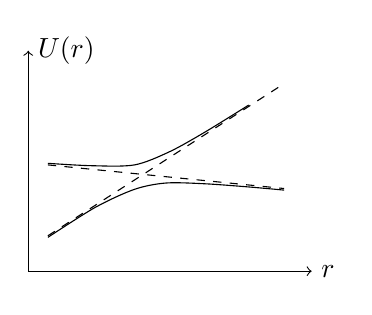
\begin{tikzpicture}[x=1cm,y=1cm]
 \draw[->] (0,0)--(3.6,0) node[right] {$r$};
 \draw[->] (0,0)--(0,2.8) node[right] {$U(r)$};
 \draw[dashed] (.25,.45)--(3.2,2.35);
 \draw[dashed] (.25,1.35)--(3.25,1.05);
 \draw[smooth] plot coordinates {(.25,1.37)(.8,1.34)(1.35,1.35)(1.8,1.52)(2.25,1.77)(2.8,2.11)};
 \draw[smooth] plot coordinates {(.25,.43)(.85,.81)(1.35,1.04)(1.75,1.12)(2.25,1.11)(2.8,1.07)(3.25,1.03)};
\end{tikzpicture}
\caption*{Fig. 27}
\end{figure}

The foregoing argument remains valid in full, except that the perturbation $\widehat V$ is now specified not by one parameter but by $s$ parameters, the displacements $\delta r_1,\ldots,\delta r_s$. With as few as two parameters, however, the two equations (79.5) can in general be satisfied. We thus conclude that in polyatomic molecules any two terms can cross. If the terms have the same symmetry, their crossing is fixed by the two conditions (79.5), and hence the dimension of the manifold along which the crossing occurs is $s-2$. If the terms have different symmetries, only one condition remains, and the crossing takes place along a manifold of $s-1$ dimensions.

Thus, when $s=2$, the terms are represented by surfaces in a three-dimensional coordinate system. For terms of different symmetry these surfaces intersect along lines ($s-1=1$), whereas for terms of the same symmetry they intersect at points ($s-2=0$). The form of the surfaces near an intersection point in the latter case is readily found. The energy values near the points where the terms cross are given by (79.4). In this expression the matrix elements $V_{11}$, $V_{22}$, $V_{12}$ are linear functions of the displacements $\delta r_1$, $\delta r_2$, and therefore also linear

\begin{figure}[ht]
\centering
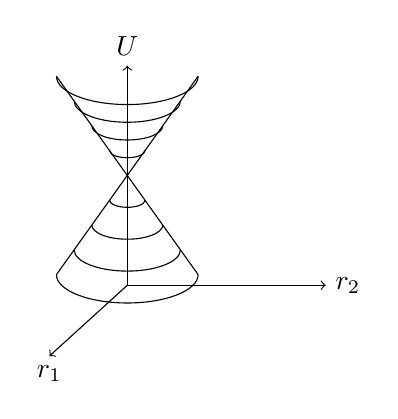
\begin{tikzpicture}[x=.9cm,y=.9cm]
 \draw[->] (0,0)--(0,3.1) node[above] {$U$};
 \draw[->] (0,0)--(2.8,0) node[right] {$r_2$};
 \draw[->] (0,0)--(-1.1,-1.0) node[below] {$r_1$};
 \foreach \h/\rx/\ry in {.35/.25/.10,.7/.5/.2,1.05/.75/.3,1.4/1/.4}
   {\draw (-\rx,1.55+\h) arc[start angle=180,end angle=360,x radius=\rx,y radius=\ry];
    \draw (-\rx,1.55-\h) arc[start angle=180,end angle=360,x radius=\rx,y radius=\ry];}
 \draw (-1,2.95)--(0,1.55)--(1,2.95);
 \draw (-1,.15)--(0,1.55)--(1,.15);
\end{tikzpicture}
\caption*{Fig. 28}
\end{figure}

\SourcePage{371}{374}
functions of the distances $r_1$, $r_2$ themselves. As is known from analytic geometry, an equation of this form describes an elliptic cone. Thus near a crossing point the terms are represented by the surface of a two-napped elliptic cone of arbitrary orientation (Fig.~28).
